\section{Fluxionnel execution model}

\subsection{Fluxions}

The fluxionnel execution model role is to manage and invoke autonomous execution units.
An execution units as we define it, accept only streams as input and output, that is a continuous and infinite sequence of data contained in messages.
We named this execution unit a fluxion.
That is a function, as in functional programming, only dependent from data streams.
It's composed of a unique name, a processing function, and a memory context during its execution.

Messages are composed of the name of the recipient fluxion, a body, and are carried by a messaging system.
% They represent both the invocation signal, and the data needed for this invocation
After processing a message, the fluxion modify its context, and then terminate its execution by sending a message on its output stream.
Each fluxion send back a unique message to one or many recipient.
The fluxion's execution context is the set of state variables whose the fluxion depends on.

The fluxions make up a chain of processing binded by data streams.
All these chains make up a directed graph, managed by the messaging system.

\subsection{Messaging system}

The messaging system is the core of our fluxionnel execution model.
Its task is both to carry messages along stream, and to invoke fluxions at a message reception.

It's build around a message queue, processed one after another by invocation of the recipient fluxion.
Using a message queue allow to execute multiple processing chain fairly and concurrently, without difference in scheduling local messages, or network messages.
The life cycle of a fluxionnel application is pictured on figure \ref{fig:MesSys}.

\begin{figure}[h!]
  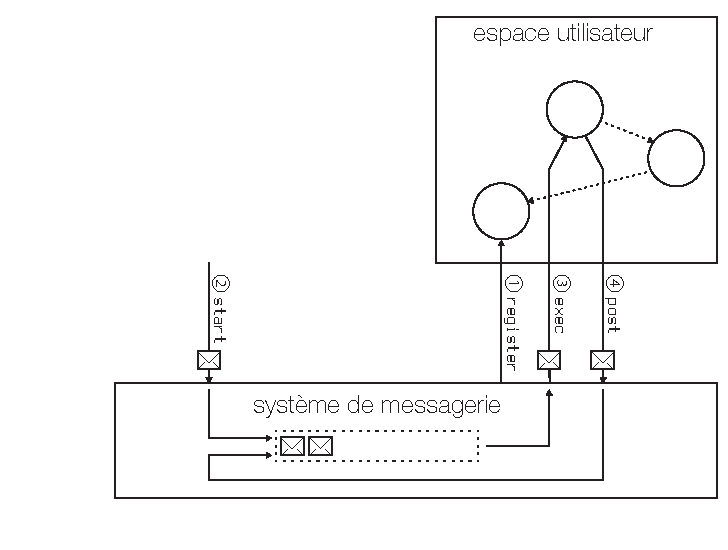
\includegraphics[width=\linewidth]{schema-message.pdf}
  \caption{Messaging system details}
  \label{fig:MesSys}
\end{figure}

The messaging system needs every fluxion to be registered.
This registration match a processing function with a unique name and an initial execution context.
The messaging system carries messages streams based on these fluxions' names.
That's why two fluxions with the same name would lead the system in a conflicting situation.
The registration is done using the function \texttt{register(<nom>, <fn>, <contexte>)}, step \circled{1} on figure \ref{fig:MesSys}.
% A fluxion can dynamically register other fluxions

To trigger a fluxions chain, a first message is sent in the messaging system, using the function \texttt{start(<msg>)}, step \circled{2}.
This function push a first message in the queue.
Immediately, the system dequeue this message to invoke the recipient processing function, step \circled{3} and \circled{4}.
The message resulting of this invocation is then enqueue on the message queue, step \circled{5} and \circled{6}.
The system loop through step \circled{3} to \circled{4} until the queue is empty.

The algorithm \ref{alg:traitement} and \ref{alg:parcours} describe precisely the behavior of the messaging system after the function \texttt{start} invocation.

\begin{algorithm}
\caption{Message queue processing algorithm}
\label{alg:traitement}
\begin{algorithmic}
\Function{processMsg}{$msg$}
\For{$dest$ \textbf{in} $msg.dest$}
\State $fluxion \gets lookup(dest)$
\State $message \gets$ \Call{exec}{$fluxion, msg.body$} \Comment{\circled{4} \& \circled{5}}
\State \Call{enqueue}{$message$} \Comment{\circled{6}}
\EndFor
\EndFunction
\end{algorithmic}
\end{algorithm}

\begin{algorithm}
\caption{Message queue walking algorithm}
\label{alg:parcours}
\begin{algorithmic}
\Function{loopMessage}{\null}
\While{$msg$ \textbf{presents in} $msgQueue$}
\State $msg \gets$ \Call{dequeue}{\null} \Comment{\circled{3}}
\State \Call{ProcessMsg}{$msg$}
\EndWhile
\EndFunction
\end{algorithmic}
\end{algorithm}

\subsection{External interfaces}

In order to interact with outside of the system, we define external border interfaces.
Our approach is based on Web architecture.
The external interface enable to communicate with a REST\footnote{REST: \textbf{Re}presentational \textbf{S}tate \textbf{T}ransfer \cite{Fielding2002}} client.
We define two components in this interface :

\begin{itemize}
	\item[\textbf{In}]
    receives client connections.
    % This is so the first link in the chain.
    For every incoming connection, this component relay a connection identifier needed by the \textbf{Out} component for the reply.
    It then relay a message the connection identifier and the request to the first fluxion in the processing chain by calling the function \texttt{start}.
	\item[\textbf{Out}]
    reply the result of the processing chain to the client.
    To receive messages from the processing chain, the component \textbf{Out} is registered in the messaging system under the name \texttt{out}.
    % This is so the last link in the chain.
\end{itemize}

The figure \ref{fig:schemaweb} pictures the specifics elements of the web interface inside the fluxionnel system.
% La figure \ref{fig:schemaweb} illustre les éléments spécifiques de cette interface Web au sein du système fluxionnel illustré par la figure \ref{fig:MesSys}.

\begin{figure}[h!]
	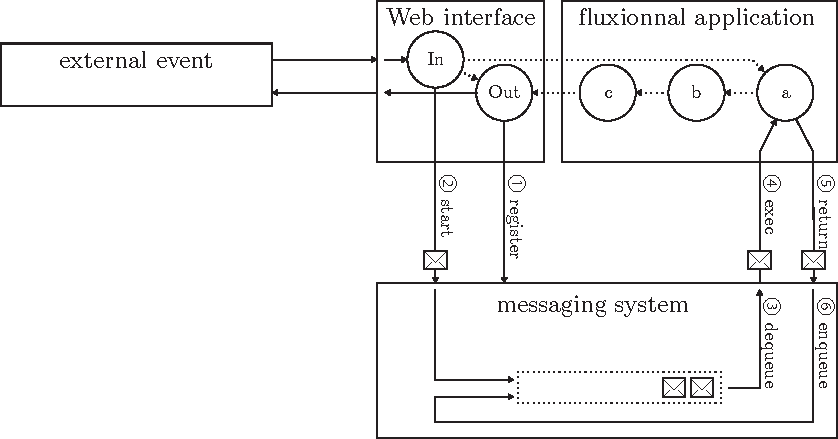
\includegraphics[width=\linewidth]{schema-web.pdf}
	\caption{Fluxionnal application with web interface}
	\label{fig:schemaweb}
\end{figure}

% TODO paragraphe de transition

\subsection{Service example}

In order to picture the fluxionnel execution model, we present in this section an example of its use with a simple visit counting service.
This service count the number of HTTP connection of each user, and send him back this number in the HTTP reply.

The inital version of this service could look like the listing extract \ref{lst:classique}.

\begin{code}[Javascript, caption={Service initial},label={lst:classique}]
var app = require('express')();

@\label{lst:classique_count}@var count = {};

@\label{lst:classique_get}\label{lst:classique_replyb}@app.get('/:id', function reply(req, res){
  count[req.params.id] = count[req.params.id]  || 1;
  ++count[req.params.id]
  var visits = count[req.params.id];
  var reply = req.params.id + ' connected ' + visits + ' times.';
@\label{lst:classique_send}@  res.send(reply);
@\label{lst:classique_replye}@});

port = 8080;
app.listen(port);
console.log("Listening port: "+port);
\end{code}

In the listing extract \ref{lst:classique}, three elements are interesting to notice.

\begin{itemize}
  \item The \texttt{count} array at line \ref{lst:classique_count} is a persistent memory to store each users visits counts under a specific user identifier.
  This array transform into a fluxion execution context in the fluxionnel system.
  \item The \texttt{reply} function, line \ref{lst:classique_replyb} to \ref{lst:classique_replye}, contains the logic we want to replace by fluxionnel processing chain.
  \item The two methods \texttt{get} and \texttt{send}, respectively line \ref{lst:classique_get} and \ref{lst:classique_send}, interface the logic and the web server.
\end{itemize}

This minimal service would be transformed with our automatic tool into the fluxions chain pictured figure \ref{fig:fluxions}.

\begin{figure}[h!]
  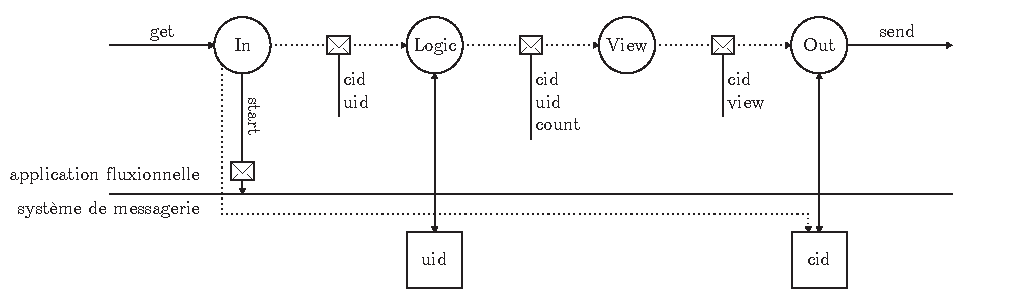
\includegraphics[width=\linewidth]{flux.pdf}
  \caption{Count service fluxions chain}
  \label{fig:fluxions}
\end{figure}

The listing extract \ref{lst:fluxionnel} describe this same counting service in a high level fluxionnel langage.
This new language bring a stricter segmentation than the initial code.
And so allow an additional system to optimize how fluxions are organized on different physical machines according to the cost of the streams and their processing. 

This high level language is not typed.
\TODO{write a paragraph about the languages caracteristics, a reserved subsection might be necessary, but maybe better placed in the next section, about transformation}

\begin{code}[Javascript, caption={Fluxionnal high level language},label={lst:fluxionnel}]
use fluxion, web

fluxion input >> view
  this.uid[msg.uid] = this.uid[msg.uid] + 1 || 1
  msg.count = this.uid[msg.uid]
  return msg

fluxion view >> output
  msg.view = msg.uid + " connected " + msg.count + " times."
  msg.uid = undefined
  msg.count = undefined
  return msg

register input, {uid: {}}
register view

web.listen
\end{code}

Except from the two interface components, the service is split as follow :
\begin{itemize}
  \item The \texttt{input} fluxion is the first to receive the client message.
  It contains the whole logic of this simple service.
  A real services would need a more complex chain with logic distributed across multiples fluxions, instead of a single fluxion.
  It increment the count for the received user identifier, push this count inside the message, and relay it the next fluxion.
  \item The \texttt{view} fluxion receive this message, and format as the user will view it, and relay it the output fluxion.
\end{itemize}